\chapter{Problem Analysis}
Accurate throughput prediction in wireless networks is inherently difficult due to the highly dynamic nature of wireless cellular networks. Given the data made available by the dataset used in this project, there were still a number of challenges that had be solved before any prediction model could be considered. This section outlines the dataset, and the understanding gleaned from it and applies this understanding to the inherent challenges faced in fitting a deep learning based throughput predictor.

\section{Outline of the Dataset}
The dataset used in this paper was collected by researchers in University College Cork in and around the greater Cork City area. Data was collected using an Android network monitoring application, G-NetTrack Pro. Apple devices currently do not have any equivalent application for collecting cellular network analytics. The dataset is a collection of 135 different traces approximately 15 minutes in length on average. Traces were collected by the UCC researchers under a number of different movement patterns. The traces are divided based on the following movement patterns:

•Static: The trace was collected while the mobile devices location remained fixed. This is characteristic of a common use case for mobile devices such as watching video while seated at a desk. Such a use case presents the best case scenario for a cellular network as the connection will experience low variability in its stability. \\
•Car: The trace was collected while travelling in Cork city and its surrounding suburbs by car. \\
•Train: The trace was collected while travelling by train. These traces contain a mix of both 4G and 3G as availability for 4G networks was in urban areas only at the time these experiments took place. \\
•Bus: Traces collected while using public transport around Cork City. \\
•Pedestrian: Traces collected while walking around Cork City center using different routes. \\

Traces were collected at a variety of times on both weekdays and weekends in order to provide adequate depiction of congestion patterns. The dataset includes of a number of physical layer metrics, as well has GPS metrics and the upload and download bitrate. The following description of the metrics collected was taken directly from the paper \cite{dataset} written by the researchers involved in the construction of this dataset. For a more in depth understanding of the dataset I recommend reading their paper. All credit goes to them for the following description of the metrics:

•Timestamp: timestamp of sample \\
•Longitude and Latitude: GPS coordinates of mobile device \\
•Velocity: velocity in kph of mobile device \\ 
•Operatorname: cellular operator name (anonymised) \\
•CellId: Serving cell for mobile device \\
•NetworkMode: mobile communication standard (2G/3G/4G) \\
•RSRQ: value for RSRQ. RSRQ Represents a ratio between RSRP and Received Signal Strength Indicator (RSSI). Signal strength (signal quality) is measured across all resource elements (RE), including interference from all sources (dB). \\
•RSRP: value for RSRP. RSRP Represents an average power over cell-specific reference symbols carried inside distinct RE. RSRP is used for measuring cell signal strength/coverage and therefore cell selection (dBm). \\
•RSSI: value for RSSI. RSSI represents a received power (wide-band) including a serving cell and interference and noise from other sources. RSRQ, RSRP and RSSI are used for measuring cell strength/coverage and therefore cell selection(handover) (dBm)0\\
•SNR: value for signal-to-noise ratio (dB). \\
•CQI: value for CQI of a mobile device. CQI is a feedback provided by UE to eNodeB. It indicates data rate that could be transmitted over a channel (highest MCS with a BLER probability less than 10\%), as the function of SINR and UE’s receiver characteristics. Based on UE’s prediction of the channel, eNodeB selects an appropriate modulation scheme and coding rate. \\
•DL\_bitrate: download rate measured at the device (application layer) (kbit/s) \\
•UL\_bitrate: uplink rate measured at the device (application layer) (kbit/s) \\
•State: state of the download process. It has two values, either I (idle, not downloading) or D (downloading) \\
•NRxRSRQ \& NRxRSRP: RSRQ and RSRP values for the neighbouring cell. \\
•Cell\_Longitude \& Cell\_Latitude: GPS coordinates of serving eNodeB. We use OpenCelliD4, the largest community open database providing GPS coordinates of cell towers. \\
•Distance: distance between the serving cell and mobile device in metres.

\newpage
\section{Considerations of the Dataset}

As the dataset is a collection of separate traces (experiments), this must be taken into account when constructing train and test splits. The entire dataset cannot be viewed as a series of disconnected time series as traces start from different physical locations, run for different lengths of time and use the same workload as a starting point for measuring network data. As such special care must be taken in order to ensure proper construction of train-test sequences.  

The dataset contains considerable missing values for some network features such as NRxRSRP \& NRxRSRQ. Lstm based machine learning techniques require complete data. As such imputation had to be carried out to fill in these gaps. There are various methods of imputation such as mean imputation, max or min imputation, K nearest neighbours (knn) based imputation \cite{batista2002study} methods and more. Some of these methods were considered in this project but it is important to note that no imputation method is perfect. Understanding of the missingness observed in the data may lead to choosing one method over the other. 

Methods like knn imputation also require considerable computational power \& space in memory compared to other more simple methods. This limits the usefulness of such a method to the training phase of a throughput predictor only. Knn or other complex imputation methods might not be viable for deployment directly on the mobile device due to the space and computational constraints of mobile devices. Edge computing would allow for more complicated imputation methods however there is also a time penalty incurred for utilising more complex methods.

Some features collected are not reported directly by the G-NetTrack Pro such as cell tower location data. As such these features were excluded from consideration in this project. If such information was made more readily available to mobile devices in the future it may prove useful in throughput prediction applications however this is outside the scope of the project.

While this dataset is robust in its construction and depiction of typical mobile communication system scenarios, it is not universal. Mobile network infrastructure implementations vary heavily by location. This dataset contains a mix of 2G/3G/4G networks. Older wireless communication technologies have different network environment distributions. As technology continues to progress the models will suffer from distribution shift. 
\newpage
\section{Identifying Missing Values}
\label{sec:missingness}
Firstly we aimed to understand the nature of missing values included in the dataset. The models considered in this paper require complete data for training. Understanding the nature of missing values in the dataset is vital in the process of selecting methods of imputation\cite{DONDERS20061087}. From figure \ref{fig:missing_bar} we observed that physical layer features SNR and CQI were unreported in approximately 30\% of sample observations with RSSI being unreported in 37\%. Cell tower related features also exhibited missing values in approximately 30\% of sample points. The degree of missingness  rules out excluding observations that containing missing values from consideration.

\begin{figure}[H]
\includegraphics[scale=0.3]{Images/missing_bar.png}
\centering
\title{Bar Chart of Missing Values}
\caption{Bar chart showing the total number of missing values for each feature over all traces.}
\label{fig:missing_bar}
\end{figure}

We then checked for correlation between observations of missing values in each column. From Figure \ref{fig:missing_heatmap} we observed a strong correlation between when the mobile device failed to report a value for the physical layer features RSSI, CQI and SNR. Geo-location data for the serving cell tower also exhibits strong positive correlation with the physical layer features. NRxRSRQ \& NRxRSRP show moderate negative correlation with for missing values with the previously mentioned features. Figure \ref{fig:missing_matrix} provides an alternative way to view these relations.

\begin{figure}[H]
\includegraphics[scale=0.3]{Images/missing_heatmap.png}
\centering
\title{Correlation of Observed Missing Values}
\caption{Correlation Heatmap for Missing values}
\label{fig:missing_heatmap}
\end{figure}

\begin{figure}[H]
\includegraphics[scale=0.3]{Images/missing_matrix.png}
\centering
\title{Visualisation of the Datasets Missing Values}
\caption{White regions indicate a missing value for that row. Diagram was sorted by RSSI to group missing rows together.}
\label{fig:missing_matrix}
\end{figure}

From this brief analysis we can conclude that the majority of the missingness observed in the dataset is MNAR (missing not at random). Attempting to impute these missing values using simple imputation methods such as mean imputation would have introduced bias into the analysis \cite{DONDERS20061087}. We concluded that figure \ref{fig:missing_matrix} identifies a reasonable cause of the missing entries. The strong positive correlation between missing values in physical layer features and the geo-location features of the serving cell suggest that the mobile device is on the edge of the current serving cell's range. This hypothesis is further reinforced by the negative correlation observed with the missing entries in neighbouring tower's physical layer features. The negative correlation suggests that neighbouring towers are more likely to be reporting values for RSRP and RSRQ when the current cell tower is not reporting values for CQI, SNR, RSSI and its geo-location data. This would make sense if the mobile device is moving into the range of a neighbouring cell tower. Assuming this hypothesis were true, it would help to inform the selection of adequate methods of imputation for each feature. This is considered in the later section \ref{sec:imputation}.

\section{Distribution of Features \& Outlier Detection}
\label{sec:dist_of_features}
The distribution of Dl\_bitrate values across all traces is shown in \ref{tab:dl_dist} with \ref{fig:dl_hist} showing the distribution of the majority of observations.

\begin{table}[!htb]
  \centering
  \caption{Distribution Statistics of Dl\_bitrate in Mbps}
  \begin{tabular}{|c|c|c|c|}
    \hline
    Mean & Standard Dev & Median & Range \\
    \hline
   10.57 & 13.82 & 5.24 & [0,168.96] \\
    \hline
  \end{tabular}
  \label{tab:dl_dist}
\end{table}

\begin{figure}[H]
\includegraphics[scale=0.7]{Images/Histogram of DL_throughput.png}
\centering
\caption{Distribution of observations of download throughput over all traces}
\label{fig:dl_hist}
\end{figure}


To show the contribution of movement patterns to the variability observed in wireless cellular network we can look at the summary statistics shown in \ref{tab:dl_dist_movement}. The "train" movement pattern experienced the lowest mean throughput. This is likely due to the reduced 4G coverage along the train's route. Following this we plotted the duration of each trace and highlighted the mean in \ref{fig:trace_length}. There is one notable outlier amongst traces who's duration is much longer than the average. This trace, trace 116, was collected while travelling by train. Because the experiment runs at least until the download of the control file is complete, it is likely that the low download throughput observed for the train mobility pattern caused this deviation.

\begin{table}[!htb]
  \centering
  \caption{Distribution Statistics of Dl\_bitrate (Mbps) per Movement Pattern}
  \begin{tabular}{|c|c|c|c|c|}
    \hline
     Movement Pattern & Mean & Standard Dev & Median & Range \\
    \hline
     Static & 10.56 & 16.66 & 3.11 & [0,95.51] \\
     Car & 13.54 & 14.19 & 9.06 & [0,144.46] \\
     Pedestrian & 10.73 & 11.79 & 6.36 & [0,77.42] \\
     Bus & 9.77 & 11.18 & 5.83 & [0,85.81] \\
     Train & 4.87 & 12.25 & 0.49 & [0,168.96] \\
    \hline
  \end{tabular}
  \label{tab:dl_dist_movement}
\end{table}

\begin{figure}[H]
\includegraphics[scale=0.7]{Images/trace_length.png}
\centering
\caption{Plot of Trace Durations}
\label{fig:trace_length}
\end{figure}

The distributions of all features were checked for normality using the shapiro-wilk normality test \cite{razali2011power}. It was found that no numeric features followed a Gaussian distribution. We then checked for outliers in each feature using the interquartile range method. $X$ is an outlier if:
\begin{equation}
X < Q1-1.5\times IQR \quad OR \quad X > Q3+1.5\times IQR
\end{equation}

A considerable number of outliers were identified in the dataset. Of the 174,523 observations, Dl\_bitrate contained 13,245 outliers. Considering nature of wireless cellular networks outliers are inevitable and as such no strict measures were taken to deal with the outliers identified. It was found the expressing some physical layer features as a weighted exponential mean of the current and previous values improved predictions slightly, and as such this was the only action taken to deal with outliers.

\section{Sequence construction}
The models were trained on input, target sequences constructed using a rolling window over the observed time series data. Sequences were created on a trace by trace basis, i.e. there is no 1 sequence that contains observations from 2 different traces.

For a given pair of input and target, the input sequence is the observed values of the predictor features over the past $p$ seconds. The target is the observed $DL\_bitrate$ of the next $k$ seconds. The variables $p$ and $k$ are referred to as the history and horizon window respectively. A single input sequence takes the shape of a [n x f] matrix where f is the no of features used to predict the target. A single target sequence takes the shape of a [k x 1] matrix as we are only interested in predicting $DL\_bitrate$. For example in the univariate case we used a history window of 10 seconds, a horizon window of 5 seconds. Previous values of $DL\_bitrate$ were used to predict the throughput horizon. E.g.
\begin{equation}
\begin{aligned}
 input&: [10 \times 1] \\
 target&: [5 \times 1]
\end{aligned}
\end{equation}

\section{Choice of History \& Horizon Windows}
A typical input for an Lstm model used in forecasting takes the shape of: $[ n, p, q ]$ where n is the number of examples, p is the length of the history window and q is the number of features. The output will then be in the form of $[n, k, s ]$ where k is the length of the horizon window and s is the number of target variables the model predicts, typically s=1. Fig \ref{fig:example_of_ts} illustrates the construction of a single example in the univariate case.

\begin{figure}[h]
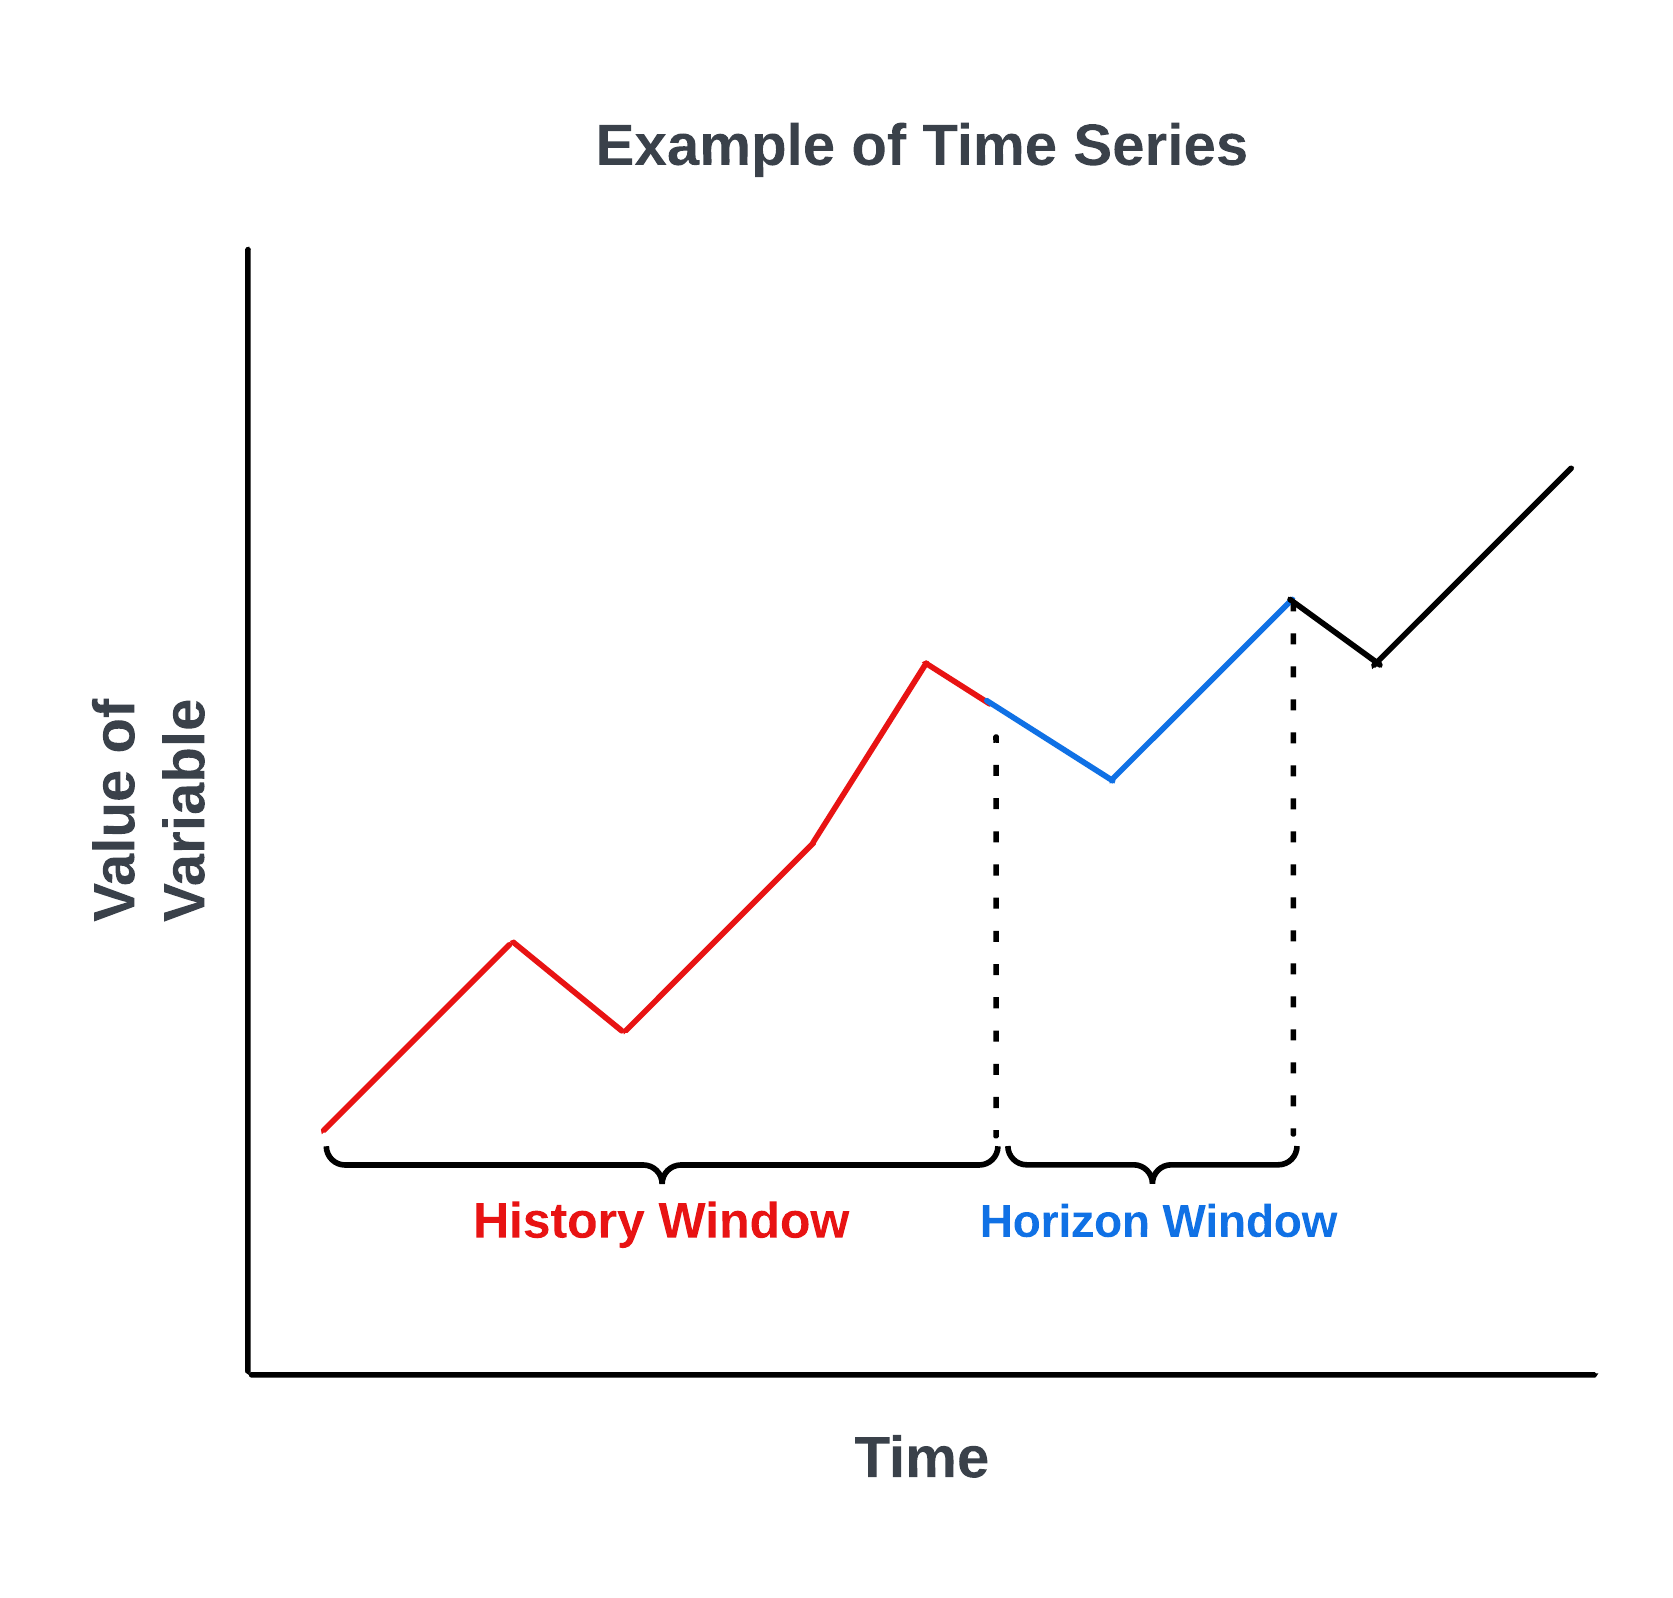
\includegraphics[scale=0.15]{History Horizon.png}
\centering
\caption{Graph showing how a history and horizon window can be constructed for a feature in time series data}
\label{fig:example_of_ts}
\end{figure}

There are many methods for identifying the optimal length of the horizon and history windows. Well studied methods such as the ACF (auto correlation function) or PACF (partial auto correlation function) \cite{10.2307/2958346} are useful for identifying temporal dependencies in the univariate case. The multivariate case is more complex as the target depends not only on previous values of itself, but previous values of other features. Still ACF provided a useful insight into the choices of history windows to consider. An ACF of <0.4 indicates that including values at the time lag does not contribute greatly to predicting the current value. An ACF >0.8 indicates that a particular lag is very relavant when predicting the current and future value of a metric.

Looking at figure \ref{fig:dl_acf} which shows the average ACF of the download throughput over the previous minute we observed that significant contributions to the prediction of current values falls off after 26 seconds. The red shaded region shows the standard deviation of the ACF observed over all traces. Intuitively this also suggests that for a horizon window of 5 seconds, 21 seconds would be an adequate maximum bound to consider for the history window.

\begin{figure}[h]
\includegraphics[scale=0.5]{Images/Average_DL_bitrate_ACF.png}
\centering
\caption{This figure shows the average value of the auto correlation function for download throughput over all traces}
\label{fig:dl_acf}
\end{figure}

A selection of different combinations of horizon and history windows were considered to evaluate the impact each has on the throughput horizon predictions, however it was found that longer horizon lengths than 15 seconds caused model performance to decrease. An important note is that the choice of history and horizon window also impacts the choice of model. The model used to test these varying windows was tuned for a window size of 10 for history and 5 for horizon. It is possible that tuning the hyper-parameters for a model with longer windows may lead to increased performance however due to computational limitations this could not be explored within the scope of the project. The horizon window is more application dependent. The granularity of data available to us through G-NetTrack Pro is one second. In general more time sensitive applications such as web-conferencing would benefit a smaller horizon window. This incurs the cost of more computational power as the throughput prediction model must be run more frequently. Inversely, less time sensitive applications could use a longer horizon window. For throughput prediction, if the average horizon throughput is the main variable of interest then a longer horizon length may actually benefit predictions as the average will be calculated over a greater number of throughput predictions \cite{raca2019improving}.

\section{Selection of train/test Splits}
Typical train/test splits divide the dataset in a given ratio, usually 80:20 for train and test respectively. This is difficult to reproduce with this dataset as the dataset is not a single continuous time series but a collection of 135 distinct time series experiments. Train and test can be created by dividing the dataset based on the number of traces however, as seen in \ref{sec:distribution} the traces are of varying length making it difficult to split the dataset based on solo on the count. Another issue is that the training set must contain an adequate count of examples for all 3 classes, low, medium and high. As the classes are imbalanced, blindly partitioning the dataset based on traces may lead to situations where all examples of a single class ends up in either the training dataset or the testing dataset. This is especially the true for low throughput examples which have the least representation in the dataset. Both the baseline model and the multistage architectures must use the same train and test in order to be comparable. Failure to provide adequate examples of each class in the training data would result in the multistage models performing poorly. Instead, division of the traces was viewed an an optimisation problem. For each trace, the number of observations for each class of low, medium and high throughput was calculated. The number of observations of each class will vary based on the chosen horizon length and as such, different choices of horizon length will require a different train and test partition. The output of this process is as follows:
\begin{table}[!htb]
  \centering
  \caption{Example of Label Counting Output}
  \begin{tabular}{|c|c|c|c|}
    \hline
    Trace No. & Low Sequence Count & Medium Sequence Count & High Sequence Count \\
    \hline
    0 & 10 & 30 & 100 \\
    1 & 4 & 32 & 70\\
    2  & 0 & 60 & 130\\
    \hline
  \end{tabular}
\end{table}
The class counts per trace were then used to calculate a percentage of the total number of observations in each class over all traces contained within each trace. These percentages are then used partition the 135 traces in a given ratio (4:1 was used) in order to achieve the desired distribution of sequences in the train/test sets. Ideally the train set would include: \\
- 80\% of all low samples, 80\% of all medium samples and 80\% of all high samples \\
- Test would be the remainder i.e 20\% of low, medium and high \\

In practice it is difficult to find a split of traces that achieves the perfect ratio between low/medium/high for train and test. Instead a large number (10000) of potential splits are created and their class \% are measured. The split that is chosen is the train/test split with the lowest sum of differences between \% training low, medium, high, that is to say, train/test split chosen has the closest distribution to the desired distribution outlined above. The preprocessing code provides a summary of the distribution of the train/test split it finds. For example, most of the analysis in this paper focuses on a history window of 10 seconds and a horizon window of 5 seconds. The distribution of the train / test split for this selection is shown in table \ref{tab:train_test_dist}. 

\begin{table}[!htb]
  \centering
  \caption{Train/Test Class Distribution}
  \npdecimalsign{.}
  \nprounddigits{5}
  \begin{tabular}{|n{1}{4}|n{1}{4}|n{1}{4}|n{1}{4}|n{1}{4}|n{1}{4}|n{1}{4}|}
    \hline
    {train low} & {train medium} & {train high} & {test low} & {test medium} & {test high} & {distribution diff} \\
    \hline
	0.8646586591494055 & 0.8362963871178682 & 0.8373981034769589 & 0.1353413408505944 & 0.1637036128821317 & 0.162601896523041 & 0.0567245440630745\\
    \hline
  \end{tabular}
  \npnoround
  \label{tab:train_test_dist}
\end{table}

\newpage
\section{Identifying Bounds for Mutlistage Model Classes}
\label{sec:bounds}
Two multistage approaches for modelling throughput prediction were considered in this paper. Each of the two architectures however share the same base models. Both multistage architectures proposed make use of a simple classifier that aims to predict a horizon throughput as one of 3 distinct situations, low throughput, medium throughput or high throughput. The choice to divide the problem based on the value of the download throughput comes from the fact that traces typically reported throughput above certain bounds (5Mbps, 1Mbps etc) far more often than below them. This imbalance leads to a single stage model frequently overestimating in low/medium throughput situations. Overestimating in these low or medium throughput scenarios leads to a noticeable decrease in the perceived quality of experience in applications such as video streaming \cite{raca2019improving} and is one of the main motivations of the multistage approach. 

The choice of the number of bounds (and subsequently models) and how to classify a given sequence of input data is arbitrary. For the purposes of this paper, dividing the data into one of three bounds sufficed. The sequences were divided by horizon download throughput into the three following ranges:

•Low:    $ mean[y] < 1Mbps$ \\
•Medium: $1Mpbs \leq mean[y] \leq 5Mpbs$ \\
•High:   $ mean[y] > 5Mbps$ \\

For forecasting, Lstm models are typically trained on x, y pairs where x is historic data of the predictor features over the past p seconds and y is the true value of the target variable of the next k seconds. The average download throughput of y was used to classify a given trace as an example of high, medium or low throughput.

The bounds 1Mbps and 5Mbps were chosen based on domain knowledge. Popular video streaming applications provide guidelines for the required download throughput for given video quality. As of the time of writing, 720p video requires 3Mbps on Netlfix whereas Youtube and Amazon Prime Video require at least 5Mbps of download throughput. While the adoption of AV1 hardware encoding may lower the required bitrate for HD video, use of the codec is still a while off mass market adoption and providers could choose to maintain the current bitrate while providing better quality source content.

\section{Feature Selection}
\label{sec:feature_selection}
Feature selection is an important step in any machine learning problem. Good feature selection is known to improve loss, increase runtime performance and improve the understandability of predictions \cite{guyon2003introduction}.
Feature selection for multivariate time series is still an evolving field. The challenge is that the a selected feature set must capture the correlation between the target variable and predictors as well as between the target variable and lagged values of the predictors.

Feature selection is important for the analysis of multistage vs single stage throughput predictors explored this paper as it is an effective method in reducing the number of parameters of a given model. This is especially important when tight constraints are put on model size (in memory) and speed of inference, as is the case for models intended for mobile devices.

The number of feature included in the dataset is relatively small at 19 by current deep learning standards. This allows for methods such as exhaustive search to be viable, however hardware limitations prevented us from carrying out such an analysis due to time constraints. Geo-location data related to the serving cell tower was excluded from consideration. This data is currently not readily available on mobile devices and had to be gathered from a third party source \href{https://opencellid.org/}.

Firstly to explore the correlation between features. Fig \ref{fig:feature_correlation} shows the average correlation matrix over all traces. The features: RSRQ, RSSI, RSRP, NRxRSRP and NRxRSRQ are measured on a logarithmic scale and as such were transformed using the following formula before calculating the correlation matrix:
\begin{equation}
Y = exp(\left|X\right|)
\end{equation}
NetworkMode\_\{X\} is the one-hot-encoded transform of the NetworkMode feature, the same is true for State\_I and State\_DBefore performing this transform correlation between DL\_bitrate and these features was not observed. Understanding this matrix requires some careful thought. Firstly, this is a time series problem, DL\_bitrate will be used to predict itself. Knowing this, the observed strong correlation between DL\_bitrate and UL\_bitrate is misleading in regards to feature selection. This matrix suggests that including UL\_bitrate might actually be redundant. SNR and CQI are good candidates for inclusion in the optimal feature subset. RSRQ and NRxRSRP are also good candidates for inclusion. RSRQ has strong correlation with both CQI and SNR suggesting that one of either SNR or CQI could be also be dropped should constraints call for it. Geo-location data had no correlation with DL\_bitrate which is to be expected as the dataset was constructed from mobile devices in a relatively small geographic area. The NetworkMode variables were one-hot encoded and as such correlation is less applicable for these features. This matrix suggests that a good feature selection would include:

-DL\_bitrate \\
-SNR \\
-CQI \\
-NRxRSRP \\
-RSRQ \\

\newpage
\begin{figure}[H]
\includegraphics[scale=0.5]{Images/feature_correlation.png}
\centering
\caption{Correlation matrix showing the average correlation between features over all traces}
\label{fig:feature_correlation}
\end{figure}

Next permutation feature importance was considered. An Lstm was fit on all network related features, as well as location data for the mobile device. The Lstm used was the standard Lstm identfied in section \ref{sec:model_tuning} The metric we chose to compare the results of this test is the mean absolute percentage error (MAPE) given by the following formula: \\

\begin{equation}
MAPE = \frac{1}{n} \times \frac{\left|true-predicted\right|}{true} \times 100
\end{equation}
where $n$ is the number of observations in the test set.

The procedure for permutation feature importance is as follows:

- Given a target variable $Y$, with predictor variables $X=\{X_1,X_2,X_3,...X_n\}$ \\
- Create a train/test split of the dataset \\
- Fit a model on the training data using all features in $X$ \\
- Compute the loss of the model on the test set to use as a baseline \\
- Randomly shuffle the values of one feature $X_k$ in the test set and compute the loss with just this feature's values shuffled. Do this $\forall X_k \in X$. \\
- Compared the performance of the model on the test set with the performance of the model on each test set with a shuffled feature \\
- Rank the features based on the difference in performance \\
- Use this ranked list to identify possible features to eliminate \\

The results of this analysis can be seen in figure \ref{fig:feature_importance}. In this case the model relied heavily on the NetworkMode feature. RSRQ was once again important in improving prediction performance. 
\newpage
\begin{figure}[H]
\includegraphics[scale=0.6]{Images/feature_importance.png}
\centering
\caption{Bar Chart showing Difference in Model Performance with Permuted Feature Column.}
\label{fig:feature_importance}
\end{figure}

\newpage
\section{Imputation \& Scaling}
\label{sec:imputation}
In section \ref{sec:missingness} we observed that the majority of missing values can be categorised as MNAR (missing not at random). The following imputation steps were considered:

- SNR: Imputed with the minimum observed value \\
- CQI: Imputed with the minimum observed value \\
- RSSI: Imputed with the minimum observed value \\
- ServingCell\_Lon: Imputed using forward fill \\
- ServingCell\_Lat: Imputed using forward fill \\
- ServingCell\_Distance: Imputed using forward fill \\
- RSRQ: Imputed using KNNImputer(k=5) from sklearn \\
- RSRP: Imputed using KNNImputer(k=5) from sklearn \\
- NRxRSRQ: Imputed using KNNImputer(k=5) from sklearn \\
- NRxRSRP: Imputed using KNNImputer(k=5) from sklearn \\


This method of imputation was compared with using the K-nearest-neighbours algorithm on all numeric features and ultimately the choice between these two methods of imputation made little to no difference in the model's performance.

As observed in section \ref{sec:dist_of_features} the distributions of features did not follow a normal distribution. Z-score based scaling works best when the data is already normally distributed. As such we chose to use min-max scaling in the range of (0,1) to preserve the actual feature distributions. Categorical features were one-hot-encoded.